Neste capítulo são descritos os vários requisitos que são necessários cumprir para cada um dos objetivos da dissertação bem como um objetivo adicional, a migração de \acrshort{http} para \acrshort{https}. Além disso, apresenta-se desde logo a arquitetura/modelo base da solução a desenvolver.

\section{Proteção da \acrshort{api} de dados}

A proteção da \acrshort{api} de dados é bastante importante visto que impede o uso indevido de pessoal não autorizado, isto é não registado. Para que um utilizador possa aceder à \acrshort{api} de dados necessita de criar uma Chave \acrshort{api} ou de pedir o registo de uma conta. A proteção da \acrshort{api} de dados da \acrshort{clav} possui os seguintes requisitos:
\begin{itemize}
    \item Todos os utilizadores devem conseguir aceder às rotas que as Chaves \acrshort{api} tem permissão de acesso
    \item Deve ser possível definir para cada rota quem pode aceder, Chaves \acrshort{api} e/ou utilizadores
    \item Se numa rota apenas podem aceder utilizadores deve ser possível definir que níveis de utilizadores podem aceder essa rota
    \item A verificação da autorização e autenticação de um pedido a uma rota é realizada a partir de um \textit{token} (\acrshort{jwt})
    \item Tanto uma Chave \acrshort{api} como um \textit{token} de utilizador são um \acrshort{jwt}
    \item Uma Chave \acrshort{api} para além de ainda ser válida (não ter expirado) deve estar ainda ativa
    \item Um utilizador desativado não pode gerar um \textit{token} de utilizador (não pode realizar \textit{login})
    \item Uma Chave \acrshort{api} deve ter a validade de 30 dias
    \item Um \textit{token} de um utilizador deve ter a validade de 8 horas
    \item A \acrshort{api} deve conseguir distinguir uma Chave \acrshort{api} de um \textit{token} de utilizador
    \item Não deve ser possível um utilizador fazer-se passar por uma Chave \acrshort{api} e vice-versa
\end{itemize}

Os pedidos a efetuar à \acrshort{api} devem possuir o \acrshort{jwt} na \textit{header} \acrshort{http} \textit{Authorization} ou na \textit{query string} do pedido em um dos seguintes campos:
\begin{itemize}[leftmargin=3cm]
    \item[\textbf{\texttt{token}}] caso seja o \texttt{token} de um utilizador:\newline
        \verb|http://example.com/path/page?token=<token>|
    \item[\textbf{\texttt{apikey}}] caso seja uma Chave \acrshort{api}:\newline
        \verb|http://example.com/path/page?apikey=<Chave API>|
\end{itemize}

Na \textit{header} \textit{Authorization} é usado o esquema de autenticação \textit{Bearer}\footnote{Mais informação em \url{https://tools.ietf.org/html/rfc6750}} com umas pequenas alterações. Portanto o conteúdo da \textit{header} \textit{Authorization}:
\begin{itemize}[leftmargin=2cm]
    \item Caso seja o \texttt{token} de um utilizador é:\newline
        \verb|token <token>|
    \item Caso seja uma Chave \acrshort{api} é:\newline
        \verb|apikey <Chave API>|
\end{itemize}
ao invés do esquema de autenticação predefinido do \textit{Bearer}: \verb|Bearer <token/Chave API>|.

Caso não seja respeitado um destes formatos, o pedido será recusado visto que a \acrshort{api} de dados não consegue identificar o \textit{token}.
Com estas duas formas de enviar o \acrshort{jwt} é possível distinguir os utilizadores das Chaves \acrshort{api} e cumprir assim um dos requisitos. Além disso, esta divisão entre utilizadores e chaves \acrshort{api} permite uma mais fácil gestão dos \textit{tokens} recebidos pela \acrshort{api} bem como permite usar duas formas diferentes de os gerar/verificar com o possível benefício de melhorar a segurança da \acrshort{api} já que também permite usar dois pares de chaves pública/privada, uma para as Chaves \acrshort{api}'s e outra para os \textit{token}'s de utilizadores impedindo assim que um utilizador se faça passar por uma chave \acrshort{api} e vice-versa. Cada par de chaves permite gerar \textit{token}'s (chave privada) e validá-los (chave pública).

Um dos requisitos é que os \textit{token}s gerados pela \acrshort{api} sejam \acrshort{jwt}s. Contudo poderiam ser outro tipo de \textit{tokens} (por exemplo uma \textit{string} aleatória e única) que o processo de envio dos \textit{tokens} para a \acrshort{api} manter-se-ia igual. Apenas seria alterada a forma de geração e verificação do \textit{token}, ou seja, uma alteração interna invisível para o utilizador.

De seguida é apresentado um diagrama com a estratégia de proteção que será implementada para cumprir os requisitos anteriormente anunciados:
\begin{figure}[H]
    \centering
    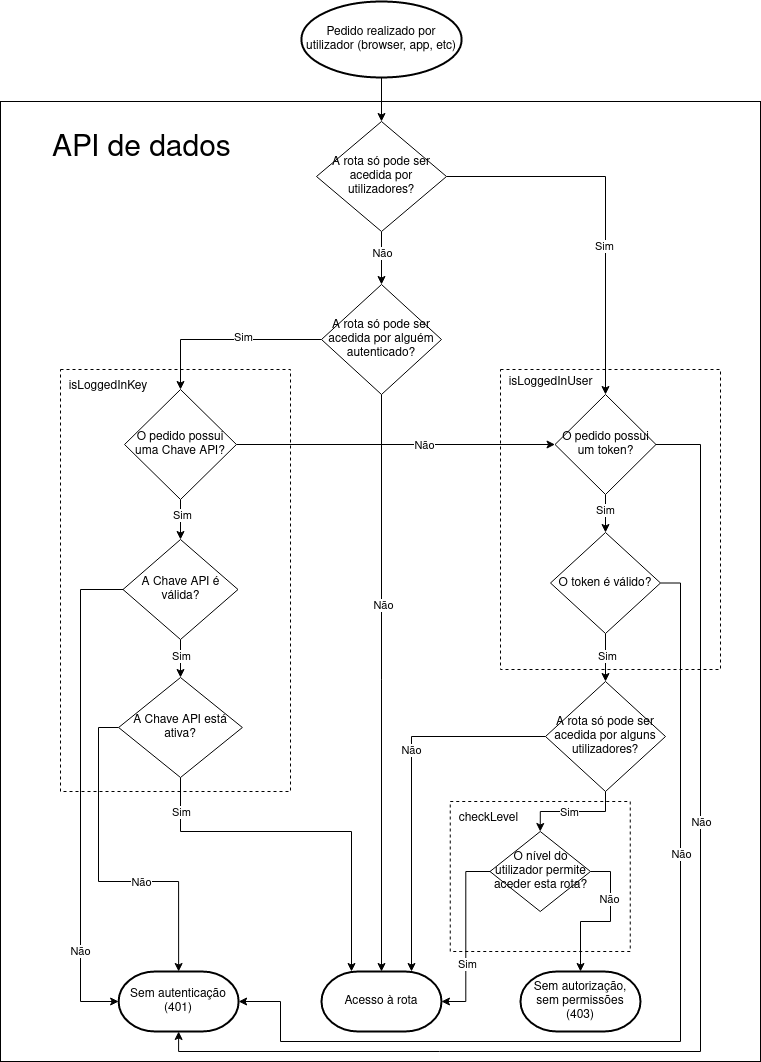
\includegraphics[width=0.7\textwidth]{img/protecaoStrag.png}
    \caption{Estratégia de proteção da \acrshort{api} de dados}\label{fig:protStrag}
\end{figure}

O \texttt{isLoggedInKey}, o \texttt{isLoggedInUser} e o \texttt{checkLevel} serão \textit{middlewares} que caso sejam usados numa rota definem desde logo quem pode aceder. Ou seja, se fou usado o \texttt{isLoggedInUser} sabe-se desde logo que apenas os utilizadores podem aceder. Por outro lado, se for usado o \texttt{isLoggedInKey} significa que podem aceder a rota as Chaves \acrshort{api} e os utilizadores. Para além disso, quando o \texttt{checkLevel} é usado após o \texttt{isLoggedInUser}, sabe-se que apenas parte dos utilizadores pode aceder, sendo que este \textit{middleware} recebe como argumento os níveis de utilizadores que podem aceder a rota. A informação do nível do utilizador está presente no \acrshort{jwt} (\textit{token}) enviado.

Cumpre-se assim, quase todos os requisitos anunciados com a exceção dos da validade dos \textit{token}'s. Estes são atingidos na geração dos \acrshort{jwt}'s no qual o \textit{token} de um utilizador é gerado para ter apenas a validade de 8 horas e uma Chave \acrshort{api} é gerada para ter a validade de 30 dias.

Após descrito como devem ser feitos os pedidos à \acrshort{api} e a estratégia de proteção a desenvolver, irá ser apresentado possíveis fluxos de interação entre utilizadores (\textit{browser}, \textit{app}, etc) e o servidor da \acrshort{api}.

O fluxo de autenticação de um utilizador na \acrshort{api} a ser implementado permite o seguinte:
\begin{figure}[H]
    \centering
    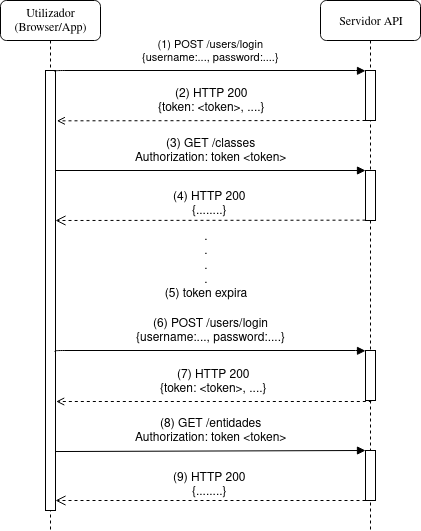
\includegraphics[width=0.5\textwidth]{img/userAuth.png}
    \caption{Fluxo de autenticação e posteriores pedidos de um utilizador}\label{fig:userAuth}
\end{figure}

\begin{enumerate}
    \item Utilizador autentica-se ao providenciar o seu \textit{email} e a sua \textit{password}
    \item Caso o utilizador se autentique com sucesso é devolvido um \textit{token} que deve ser usado nos restantes pedidos até expirar
    \item Utilizador realiza um pedido para obter as classes, colocando o \textit{token} na \textit{header} \textit{Authorization}
    \item Caso o \textit{token} enviado seja válido e não tenha expirado são devolvidas as classes
    \item \textit{Token} expirou após o tempo definido
    \item Utilizador realiza uma nova autenticação por forma a obter um novo \textit{token}
    \item Caso o utilizador se autentique com sucesso é devolvido um \textit{token} que deve ser usado nos restantes pedidos até expirar
    \item Utilizador realiza um pedido para obter as entidades, colocando o \textit{token} na \textit{header} \textit{Authorization}
    \item Caso o \textit{token} enviado seja válido e não tenha expirado são devolvidas as entidades
\end{enumerate}

O fluxo de autenticação e renovação de uma Chave \acrshort{api} na \acrshort{api} a ser implementado permite o seguinte:
\begin{figure}[H]
    \centering
    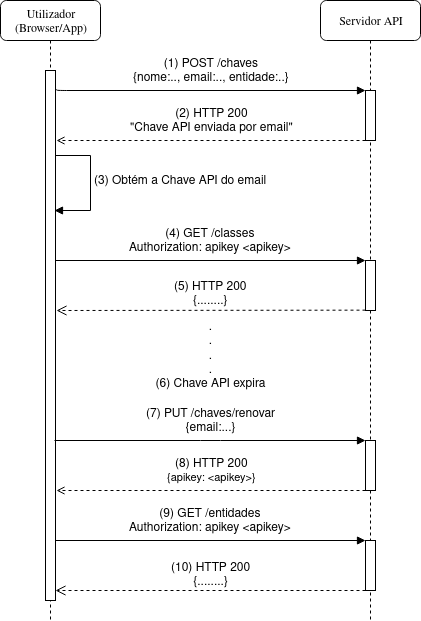
\includegraphics[width=0.5\textwidth]{img/chaveAuth.png}
    \caption{Fluxo de autenticação e posteriores pedidos de uma chave \acrshort{api}}\label{fig:chaveAuth}
\end{figure}

\begin{enumerate}
    \item Utilizador cria uma chave \acrshort{api} ao providenciar o nome, email e entidade
    \item A Chave \acrshort{api} é enviada para o email fornecido pelo utilizador com o objetivo de ser usada nos próximos pedidos
    \item O utilizador obtém a chave \acrshort{api} do email enviado
    \item Utilizador realiza um pedido para obter as classes, colocando a chave \acrshort{api} na \textit{header} \textit{Authorization}
    \item Caso a Chave \acrshort{api} enviada seja válida e não tenha expirado são devolvidas as classes
    \item Chave \acrshort{api} expirou após o tempo definido
    \item Utilizador renova a Chave \acrshort{api} ao providenciar o email usado para criar a Chave \acrshort{api}
    \item A nova (renovada) Chave \acrshort{api} é devolvida para ser usada nos restantes pedidos
    \item Utilizador realiza um pedido para obter as entidades, colocando a Chave \acrshort{api} na \textit{header} \textit{Authorization}
    \item Caso a Chave \acrshort{api} enviada seja válida e não tenha expirado são devolvidas as entidades
\end{enumerate}

\section{Autenticação através de \acrshort{cmd}}

A autenticação com \acrshort{cmd} é bastante semelhante à autenticação com o \acrshort{cc}. O que muda é o modo de autenticação perante o Autenticação.gov que em vez de ser efetuado com \acrshort{cc} (\acrlong{cc}, Leitor de Cartões, \textit{software} local do Autenticação.gov e \acrshort{pin} de autenticação do \acrshort{cc}) será realizado através de \acrshort{cmd} (Número de telemóvel, \acrshort{pin} definido durante a ativação da \acrshort{cmd} e \acrshort{pin} temporário enviado para o número de telemóvel).

Os atributos pedidos ao Autenticação.gov são os mesmos que são pedidos com a autenticação com o \acrshort{cc} (\acrshort{nic} e Nome Completo) permitindo identificar unicamente o utilizador a partir do \acrshort{nic}. Para além disso, permite aproveitar todo o back-end e código já desenvolvido para a autenticação do utilizador perante a \acrshort{clav} através de \acrshort{cc} visto que os atributos usados são os mesmos. Além disso, permite uma melhor normalização da identificação dos utilizadores (não existindo assim vários ids para o mesmo utilizador) bem como evita ser necessário o utilizador partilhar atributos adicionais (como o número de telemóvel) com a \acrshort{clav} (o número de telemóvel é apenas partilhado com o Autenticação.gov sendo que a \acrshort{clav} não tem acesso a esta informação se apenas pediu para saber os atributos \acrshort{nic} e Nome Completo). Assim, a única implicação que pode ser gerada daqui é que o utilizador, quer queira usar a autenticação por \acrshort{cc} quer queira usar por \acrshort{cmd}, necessita de estar registado na \acrshort{clav} com o \acrshort{cc} sendo que, neste momento é obrigatório o registo dos utilizadores através de \acrshort{cc}. Voltasse a frisar que o \acrshort{nic} será usado por forma a identificar o utilizador, pelo que serve de id do utilizador tal como na autenticação com o \acrshort{cc}.

Portanto, de igual forma como na autenticação com o \acrshort{cc}, quando é selecionado este método de autenticação, a \acrshort{clav} redireciona o utilizador para o Autenticação.gov que se encarrega de autenticar o utilizador com \acrshort{cmd}, comunicando, no fim, os atributos pedidos ao Autenticação.gov (\acrshort{nic} e Nome Completo). A \acrshort{clav} com o \acrshort{nic} verifica se o utilizador já se encontra registado, obtendo mais alguma informação adicional, como o nível de utilizador. Semelhantemente à autenticação local e à autenticação com o \acrshort{cc}, é agora gerado um \textit{token} (\acrshort{jwt}) que irá assinar a partir daqui todos os pedidos do utilizador. O \textit{token} tem a validade de 8 horas, ao fim das quais o utilizador necessita de realizar uma nova autenticação.

Em termos técnicos, é apenas necessário aproveitar o pedido POST que já é enviado ao Autenticação.gov para a autenticação com \acrshort{cc} e adicionar as extensões nível de confiança e a política de apresentação como é possível constatar em~\ref{sec:soaAuthCMDReq}.

A primeira extensão permite indicar o nível mínimo necessário que pretendemos que seja usado pelo Autenticação.gov. Como tal, dado um nível selecionado permite a autenticação através do método desse nível mas também permite os métodos de autenticação dos níveis superiores. Além disso, quanto menor o nível mais fraca é a autenticação, visto que quanto menor o nível mais fraca é a autenticidade das credenciais fornecidas pelo utilizador.

Quando este nível de confiança não está presente (como no caso do pedido enviado para a autenticação com \acrshort{cc}) o nível de confiança mínimo assumido é o nível máximo (4). Assim para o caso da \acrshort{cmd} será adicionada a seguinte extensão ao pedido em XML~\cite{agov2}:
%Ref: Manual de Integração do Fornecedor de Autenticação v1.5.3 cap 7.2
\begin{lstlisting}[language=xml, caption=Extensão Nível de Confiança no pedido enviado ao Autenticação.gov]
<fa:FAAALevel xmlns:fa="http://autenticacao.cartaodecidadao.pt/atributos">
    3
</fa:FAAALevel>
\end{lstlisting}
Esta extensão indica então que o nível de confiança mínimo necessário é o nível 3, ou seja, permite a autenticação através de \acrshort{cmd} mas também através de \acrshort{cc}.

Como tal, por forma a apenas aparecer no Autenticação.gov a hipótese de autenticação através de \acrshort{cmd} é necessário definir a Política de Apresentação do Autenticação.gov.

Ou seja, é necessário esconder a aba do \acrfull{cc} e se futuramente se pretender apresentar ambas as abas é também necessário tornar o mecanismo de \acrfull{cmd} a aba predefinida. Para tal, foi adicionada a seguinte extensão ao pedido em XML~\cite{agov2}:
%Ref: Manual de Integração do Fornecedor de Autenticação v1.5.3 cap 8.2
\begin{lstlisting}[language=xml, caption=Extensão Política de Apresentação no pedido enviado ao Autenticação.gov]
<fa:AuthTabPresentationPolicies xmlns:fa="http://autenticacao.cartaodecidadao.pt/presentationpolicy">
    <!--Torna a aba CMD como predefinida-->
    <fa:defaultSelectedAuthTab TabId="CMD"/>
    <!--Esconde a aba do CC-->
    <fa:hideAuthTab TabId="CC"/> 
</fa:AuthTabPresentationPolicies>
\end{lstlisting}
em que torna a aba do mecanismo de \acrshort{cmd} o predefinido e esconde a aba do mecanismo de \acrshort{cc}.

Portanto, se for enviado um pedido ao Autenticação.gov igual ao da autenticação com \acrshort{cc} mas com estas extensões, o Autenticação.gov pedirá ao utilizador para se autenticar com \acrshort{cmd}.

\section{Documentação da \acrshort{api} da \acrshort{clav}}

No estado da arte foram abordadas várias alternativas ao \textit{Swagger UI}. A partir da tabela~\ref{table:swaggerUI} e tendo em conta que:
\begin{itemize}
    \item Não há financiamento
    \item Já existe uma \acrshort{api} desenvolvida
    \item A documentação deve estar acessível de um domínio próprio
    \item A documentação deve ser fácil de criar, de editar e de manter
    \item Será usada a especificação \textit{OpenAPI}
\end{itemize}

as várias alternativas ficam reduzidas ao \textit{Swagger \acrshort{ui}} e ao \textit{ReDoc}. Optou-se por escolher o \textit{Swagger \acrshort{ui}} visto ser a ferramenta mais amplamente usada para além de que é possível obter também uma fácil integração no \textit{Swagger \acrshort{ui}} com recurso à \textit{package} \texttt{swagger-ui-express} já aprofundada no estado da arte (ver~\ref{sec:soaDocAPI}). Além disso, escolheu-se a \textit{package} \texttt{yaml-include} por forma a auxiliar a produção da documentação na criação do ficheiro com a especificação \textit{OpenAPI}, permitindo que esta documentação seja modular.

A documentação modular será estruturada da seguinte forma:

\begin{lstlisting}[caption=Excerto da estrutura modular da documentação]
* /index.yaml
* /paths/
    * /classes/
        * /get.yaml
        * /post.yaml
        * /~id/
            * /get.yaml
            ...
        ...
    ...
* /examples/
    * /classes/
        * /ClasseCompletaJSON.yaml
        * /ClasseCompletaXML.yaml
        * /ClasseSimplesJSON.yaml
        ...
    ...
* /schemas/
    * /classes/
        * /ClasseCompleta.yaml
        ...
    * /definicoes/
        * Codigo.yaml
        ...
    ...
\end{lstlisting}

Portanto nesta estrutura na pasta \texttt{paths} é seguida a estrutura do \texttt{yaml-include} já descrita no estado da arte em~\ref{exem:faf} em que as pastas indicam o caminho e o nome dos ficheiros o verbo \acrshort{http} da rota. Em cada um destes ficheiros é colocada a descrição, os parâmetros, etc, da rota. Nestes ficheiros serão feitas referências aos \texttt{schemas} e \texttt{examples} necessários, estando estes nas pastas \texttt{schemas} e \texttt{examples} respetivamente. Isto permite que os modelos e os exemplos sejam reutilizados para além de que permite tornar os ficheiros onde são referenciados mais fáceis de perceber, principalmente em casos em que os modelos e os exemplos são extensos.

Em termos de organização das pastas \texttt{schemas} e \texttt{examples}, estas no primeiro ``nível'' possuem pastas de cada grupo de rotas (classes, entidades, \textit{users}, chaves, etc) e em cada uma destas pastas estão os modelos/exemplos correspondentes a esse grupo de rotas. Na pasta \texttt{schemas} existe contudo uma pasta especial chamada \texttt{definicoes} que possui os vários tipos de dados, como por exemplo o código de uma classe, o id de uma entidade, etc. Assim, estes modelos são usados nos outros modelos e nas rotas permitindo uniformizar estes dados. Ou seja, caso haja por exemplo alguma alteração no formato do código, será apenas necessário alterar no modelo presente na pasta \texttt{definicoes} que a alteração será ``propagada'' já que todos que precisam deste modelo fazem-lhe referência. Portanto, sempre que é criado um novo modelo ou uma nova rota, convém verificar nesta pasta \texttt{definicoes} se já existe o tipo de dados necessário a usar bastando assim fazer-lhe referência.

Por fim, no ficheiro \texttt{index.yaml} é definido os grupos de rotas (\textit{tags}) bem como várias informações gerais sobre a \acrshort{api} de dados, como descrição, métodos de autenticação, etc. Além disso, é aqui também definido, apenas no caso da pasta \texttt{examples}, que ficheiros deve o \texttt{yaml-include} ignorar ao incluir a pasta \texttt{examples} sobre a \textit{tag} \texttt{examples} dos \texttt{components}. Isto é efetuado por forma a evitar erros de sintaxe da especificação \textit{OpenAPI}. Estes erros acontecem porque há vários ficheiros de exemplos a serem incluídos nos ficheiros das rotas diretamente pelo \texttt{yaml-include} em vez de se usar o \verb|$ref| da especificação \textit{OpenAPI} em casos que o \verb|$ref| não permite efetuar o pretendido. Assim, estes ficheiros têm de ser ignorados.

Com o \texttt{yaml-include}, sempre que a \acrshort{api} de dados inicia é criado o ficheiro de especificação \textit{OpenAPI} final que incluirá os dados destes ficheiros nos seus locais apropriados. Este ficheiro final ficará disponível na pasta pública do servidor com o nome \texttt{clav.yaml} ou seja acessível a partir de \url{http://clav-api.dglab.gov.pt/clav.yaml}. É este o ficheiro que alimenta o \textit{SwaggerUI} construído com o \textit{swagger-ui-express} e disponível em \url{http://clav-api.dglab.gov.pt/v2/docs}.

\section{Exportação de dados}

Nesta secção será apresentado a especificação dos documentos finais das exportações a realizar, decidindo se algumas das bibliotecas apontadas no estado da arte (\ref{sec:exportacao}) permitem auxiliar ou realizar as conversões necessárias.

\subsection{\acrshort{xml}}

De seguida, apresenta-se a especificação do documento final em \acrshort{xml}:
\begin{itemize}
    \item Os dados exportados devem ser encapsulados com a \textit{tag} \texttt{root} por forma a garantir que só existe um elemento \textit{root} no documento \acrshort{xml} gerado respeitando as regras do \acrshort{xml}
    \item Para cada tipo de dados do \acrshort{json} deve ser convertido da seguinte forma:
    \begin{itemize}
        \item \textit{string}: Manter-se igual tirando os caracteres ``\texttt{<}'', ``\texttt{>}'', ``\texttt{\&}'', ``\texttt{'}'' e ``\texttt{"}'' que devem ser convertidos para a \textit{Entity Reference}\footnote{``\texttt{<}'' para ``\texttt{\&lt;}'', ``\texttt{>}'' para ``\texttt{\&gt;}'', ``\texttt{\&}'' para ``\texttt{\&amp;}'', ``\texttt{'}'' para ``\texttt{\&apos;}'' e ``\texttt{"}'' para ``\texttt{\&quot;}''} correspondente
        \item \textit{number}: Manter-se igual
        \item \textit{boolean}: Manter-se igual
        \item \textit{null}: Origina uma \textit{string} vazia
        \item \textit{array}: Cada item do \textit{array} deve ser encapsulado numa \textit{tag} \texttt{item} que possui um atributo \texttt{index} que indica a posição do elemento no \textit{array} e um atributo \texttt{type} que indica o tipo do elemento do \textit{array}. O tipo pode ser \textit{number}, \textit{boolean}, \textit{string}, \textit{array} ou \textit{object}.
        \item \textit{object}: Para cada propriedade deve ser criado uma \textit{tag} com valor igual à chave da propriedade e ao valor da propriedade deve ser aplicado recursivamente uma das transformações desta lista. Esta \textit{tag} deve ter um atributo \texttt{type} em que o seu valor, tal como nos \textit{arrays}, pode ser \textit{number}, \textit{boolean}, \textit{string}, \textit{array} ou \textit{object}.
    \end{itemize}
\end{itemize}

Depois de compreendida a especificação se observarmos as bibliotecas exploradas na secção do estado da arte percebemos que não há nenhuma que permita obter esta especificação sem alterar o objeto \acrshort{json} a exportar (a converter) o que acaba por em certas situações ser mais complicado do que construir um conversor específico para esta especificação. Assim, decidiu-se que seria criado um conversor de \acrshort{json} para \acrshort{xml}.

\subsection{\acrshort{csv}}

O documento \acrshort{csv} exportado deve respeitar a seguinte especificação:
\begin{itemize}
    \item O conjunto de objetos permitidos é lista de classes, de entidades, de tipologias e de legislações e objeto de classe, de entidade, de tipologia e de legislação.
    \item A conversão das listas de classes, de entidades, de tipologias e de legislações deve ter a presença dos títulos na primeira linha e depois um elemento por linha.
    \item Todos os valores das propriedades tem de ser encapsulados com aspas (\verb|"|)
    \item Os valores de uma linha devem ser concatenados com ponto e vírgula (\verb|;|)
    \item As linhas devem ser concatenadas com nova linha (\verb|\n|)
    \item Caso o valor de uma propriedade a converter seja uma lista, a conversão a realizar irá depender da propriedade e do objeto que está a ser convertido: 
    \begin{itemize}
        \item Num objeto Classe:
        \begin{itemize}
            \item Propriedade `notasAp':
            \begin{itemize}
                \item Título: Notas de aplicação \\
                      Valor: Concatenação por \verb|#\n| da propriedade `nota' de cada elemento da lista
            \end{itemize}
            \item Propriedade `exemplosNotasAp':
            \begin{itemize}
                \item Título: Exemplos de NA \\
                      Valor: Concatenação por \verb|#\n| da propriedade `exemplo' de cada elemento da lista
            \end{itemize}
            \item Propriedade `notasEx':
            \begin{itemize}
                \item Título: Notas de exclusão \\
                      Valor: Concatenação por \verb|#\n| da propriedade `nota' de cada elemento da lista
            \end{itemize}
            \item Propriedade `termosInd':
            \begin{itemize}
                \item Título: Termos Indice \\
                      Valor: Concatenação por \verb|#\n| da propriedade `termo' de cada elemento da lista
            \end{itemize}
            \item Propriedade `donos':
            \begin{itemize}
                \item Título: Donos do processo \\
                      Valor: Concatenação por \verb|#\n| da propriedade `sigla' de cada elemento da lista
            \end{itemize}
            \item Propriedade `participantes', gera duas colunas no \acrshort{csv}:
            \begin{itemize}
                \item Título: Participante no processo \\
                      Valor: Concatenação por \verb|#\n| da propriedade `sigla' de cada elemento da lista
                \item Título: Tipo de intervenção do participante \\
                      Valor: Concatenação por \verb|#\n| da propriedade `participLabel' de cada elemento da lista
            \end{itemize}
            \item Propriedade `processosRelacionados', gera três colunas no \acrshort{csv}:
            \begin{itemize}
                \item Título: Código do processo relacionado \\
                      Valor: Concatenação por \verb|#\n| da propriedade `codigo' de cada elemento da lista
                \item Título: Título do processo relacionado \\
                      Valor: Concatenação por \verb|#\n| da propriedade `titulo' de cada elemento da lista
                \item Título: Tipo de relação entre processos \\
                      Valor: Concatenação por \verb|#\n| da propriedade `idRel' de cada elemento da lista
            \end{itemize}
            \item Propriedade `legislacao', gera duas colunas no \acrshort{csv}:
            \begin{itemize}
                \item Título: Diplomas jurídico-administrativos REF Ids \\
                      Valor: Concatenação por \verb|#\n| da propriedade `idLeg' de cada elemento da lista
                \item Título: Diplomas jurídico-administrativos REF Títulos \\
                      Valor: Cada elemento da lista é mapeado para a concatenação da propriedade `tipo' com a propriedade `numero' com um espaço entre as duas propriedades; Concatenação por \verb|#\n| do mapeamento de cada elemento da lista
            \end{itemize}
            \item Propriedade `filhos': cada elemento deve ser convertido como se tratasse de um objeto classe; Deve ser ignorado os títulos gerados, mantendo apenas os valores numa nova linha do \acrshort{csv}
        \end{itemize}
        \item Num objeto Entidade:
        \begin{itemize}
            \item Propriedade `dono':
            \begin{itemize}
                \item Título: Dono no processo \\
                      Valor: Concatenação por \verb|#\n| da propriedade `codigo' de cada elemento da lista
            \end{itemize}
            \item Propriedade `participante', gera duas colunas no \acrshort{csv}:
            \begin{itemize}
                \item Título: Participante no processo \\
                      Valor: Concatenação por \verb|#\n| da propriedade `codigo' de cada elemento da lista
                \item Título: Tipo de intervenção no processo \\
                      Valor: Concatenação por \verb|#\n| da propriedade `tipoPar' de cada elemento da lista
            \end{itemize}
            \item Propriedade `tipologias':
            \begin{itemize}
                \item Título: Tipologias da entidade \\
                      Valor: Concatenação por \verb|#\n| da propriedade `sigla' de cada elemento da lista
            \end{itemize}
        \end{itemize}
        \item Num objeto Tipologia:
        \begin{itemize}
            \item Propriedade `entidades':
            \begin{itemize}
                \item Título: Entidades da tipologia \\
                      Valor: Concatenação por \verb|#\n| da propriedade `sigla' de cada elemento da lista
            \end{itemize}
            \item Propriedade `dono':
            \begin{itemize}
                \item Título: Dono no processo \\
                      Valor: Concatenação por \verb|#\n| da propriedade `codigo' de cada elemento da lista
            \end{itemize}
            \item Propriedade `participante', gera duas colunas no \acrshort{csv}:
            \begin{itemize}
                \item Título: Participante no processo \\
                      Valor: Concatenação por \verb|#\n| da propriedade `codigo' de cada elemento da lista
                \item Título: Tipo de intervenção no processo \\
                      Valor: Concatenação por \verb|#\n| da propriedade `tipoPar' de cada elemento da lista
            \end{itemize}
        \end{itemize}
        \item Num objeto Legislação:
        \begin{itemize}
            \item Propriedade `entidades':
            \begin{itemize}
                \item Título: Entidades \\
                      Valor: Concatenação por \verb|#\n| da propriedade `sigla' de cada elemento da lista
            \end{itemize}
            \item Propriedade `regula':
            \begin{itemize}
                \item Título: Regula processo \\
                      Valor: Concatenação por \verb|#\n| da propriedade `codigo' de cada elemento da lista
            \end{itemize}
        \end{itemize}
        \item Na propriedade `pca' de um objeto Classe:
        \begin{itemize}
            \item Propriedade `justificacao', gera duas colunas no \acrshort{csv}:
            \begin{itemize}
                \item Título: Critério PCA \\
                      Valor: Concatenação por \verb|#\n| da propriedade `tipoId' de cada elemento da lista
                \item Título: ProcRefs/LegRefs PCA \\
                      Valor: Cada elemento da lista é mapeado para a concatenação por \verb|#\n| da lista presente na propriedade `processos' ou na propriedade `legs' sendo a concatenação encapsulada por parênteses curvos; Concatenação por \verb|#\n| do mapeamento de cada elemento da lista               
            \end{itemize}
        \end{itemize}
        \item Na propriedade `df' de um objeto Classe:
        \begin{itemize}
            \item Propriedade `justificacao', gera duas colunas no \acrshort{csv}:
            \begin{itemize}
                \item Título: Critério DF \\
                      Valor: Concatenação por \verb|#\n| da propriedade `tipoId' de cada elemento da lista
                \item Título: ProcRefs/LegRefs DF \\
                      Valor: Cada elemento da lista é mapeado para a concatenação por \verb|#\n| da lista presente na propriedade `processos' ou na propriedade `legs' sendo a concatenação encapsulada por parênteses curvos; Concatenação por \verb|#\n| do mapeamento de cada elemento da lista               
            \end{itemize}
        \end{itemize}
    \end{itemize}
    \item Caso o valor de uma propriedade seja um objeto, as propriedades do objeto aninhado devem ser processadas como se tratassem de propriedades do objeto possuidor da propriedade com o objeto aninhado
    \item Nos casos em que o valor não é uma lista nem um objeto deve ser mantido o valor (apenas encapsulado por \verb|"|) e associado o seguinte título:
    \begin{itemize}
        \item Num objeto Classe:
        \begin{itemize}
            \item Propriedade `codigo': Código
            \item Propriedade `titulo': Título
            \item Propriedade `descricao': Descrição
            \item Propriedade `tipoProc': Tipo de processo
            \item Propriedade `procTrans': Processo transversal (S/N)
        \end{itemize}
        \item Num objeto Entidade:
        \begin{itemize}
            \item Propriedade `sigla': Sigla
            \item Propriedade `designacao': Designação
            \item Propriedade `estado': Estado
            \item Propriedade `sioe': ID SIOE
            \item Propriedade `internacional': Internacional
        \end{itemize}
        \item Num objeto Tipologia:
        \begin{itemize}
            \item Propriedade `sigla': Sigla
            \item Propriedade `designacao': Designação
            \item Propriedade `estado': Estado
        \end{itemize}
        \item Num objeto Legislação:
        \begin{itemize}
            \item Propriedade `tipo': Tipo
            \item Propriedade `numero': Número
            \item Propriedade `data': Data
            \item Propriedade `sumario': Sumário
            \item Propriedade `fonte': Fonte
            \item Propriedade `link': Link
        \end{itemize}
        \item Na propriedade `pca' de um objeto Classe:
        \begin{itemize}
            \item Propriedade `valores': Prazo de conservação administrativa
            \item Propriedade `notas': Nota ao PCA
            \item Propriedade `formaContagem': Forma de contagem do PCA
            \item Propriedade `subFormaContagem': Sub Forma de contagem do PCA
        \end{itemize}
        \item Na propriedade `df' de um objeto Classe:
        \begin{itemize}
            \item Propriedade `valor': Destino Final
            \item Propriedade `notas': Notas ao DF
        \end{itemize}
    \end{itemize}
    \item Na exportação para Excel as concatenações \verb|#\n| devem ser apenas \verb|#|
    \item As propriedades não referidas nesta especificação devem ser ignoradas
\end{itemize}

A partir da especificação e olhando para as bibliotecas de conversão exploradas no estado da arte chegou-se à conclusão que não havia nenhuma biblioteca que contivesse todas as funcionalidades necessárias. Contudo, é importante assinalar que a biblioteca \texttt{json2csv} possui grande parte das funcionalidades necessárias permitindo respeitar grande parte da especificação. Apesar disso, não é possível respeitar ``\textit{Propriedade `filhos': cada elemento deve ser convertido como se tratasse de um objeto classe; Deve ser ignorado os títulos gerados, mantendo apenas os valores numa nova linha do \acrshort{csv}''}. Além disso, o uso da biblioteca em questão obrigaria à criação de várias funções de transformação de dados por forma a respeitar a especificação. Por estas duas razões, decidiu-se que era mais conveniente, mais rápido e mais fácil criar um conversor próprio de \acrshort{json} para \acrshort{csv}.

\subsection{Ontologia}

Por fim quanto à exportação da ontologia, das três é a mais simples visto que o \textit{GraphDB} como já se referiu no estado da arte, possui funcionalidades de exportação dos triplos de uma \acrshort{bd}. Assim, apenas é necessário realizar um pedido à \acrshort{api} de dados indicando no cabeçalho \textit{Accept} do pedido o formato de saída.

Esta rota da \acrshort{api} possui vários formatos de exportação pelo que se decidiu suportar na \acrshort{api} da \acrshort{clav} apenas as mais populares.

Portanto, dos vários formatos de serialização \acrshort{rdf} serão apenas suportados (acessíveis) na \acrshort{clav}, o \acrshort{turtle} (\texttt{text/turtle}), o \acrshort{json-ld} (\texttt{application/ld+json}) e o \acrshort{rdf}/\acrshort{xml} (\texttt{application/rdf+xml}).

Apesar da facilidade de exportação da ontologia estes pedidos de exportação originam um grande consumo de recursos de \textit{hardware} por parte do \textit{GraphDB} visto que cada pedido devolve todos os triplos de uma \acrshort{bd} (a atual \acrshort{bd} da \acrshort{clav} possui já cerca de 150 000 triplos explícitos e cerca de 85 000 triplos implícitos) para além da conversão necessária desses triplos para o formato de serialização \acrshort{rdf} de saída. Deve-se então limitar o número de pedidos de exportação realizados ao \textit{GraphDB}. Para tal irá ser usado o seguinte mecanismo de controlo/\textit{cache}:\label{sec:expOntCache}

\begin{itemize}
    \item Os ficheiros exportados são mantidos pela \acrshort{api} da \acrshort{clav}
    \item Mantém-se dois ficheiros por cada serialização \acrshort{rdf}, um com os triplos explícitos e outro com os triplos explícitos e implícitos.
    \item Se o ficheiro pretendido não existe na \acrshort{api} da \acrshort{clav} realiza-se o pedido de exportação ao \textit{GraphDB}
    \item Se o ficheiro pretendido existe na \acrshort{api} da \acrshort{clav} mas não é atualizado há sete dias realiza-se o pedido de exportação ao \textit{GraphDB}
    \item Se o ficheiro pretendido existe na \acrshort{api} da \acrshort{clav} e foi atualizado há menos de sete dias devolve-se ao utilizador o ficheiro guardado na \acrshort{api} da \acrshort{clav}
    \item Mantém-se na \acrshort{api} da \acrshort{clav} apenas o ficheiro mais recente para cada versão de cada serialização \acrshort{rdf}
    \item Cada ficheiro é apenas atualizado (removendo o antigo) quando é feito um pedido por um utilizador desse ficheiro
\end{itemize}

Assim, respeitando todas estas restrições, são mantidas pela \acrshort{api} da \acrshort{clav} no máximo seis ficheiros, dois por cada serialização \acrshort{rdf}. Para além disso estes ficheiros são atualizados no melhor caso de sete em sete dias e no pior caso nunca se o ficheiro nunca for requisitado pelos utilizadores.

\subsection{Exportação na \acrshort{api} de dados}
Nesta secção será explicado de que forma será possível exportar os dados da \acrshort{api}. Para tal definiu-se a \textit{query string} \texttt{fs} (formato de saída) onde é possível indicar claro está o formato de saída. Esta \textit{query string} estará presente nas rotas onde será possível exportar os dados. Para além disso, nestas rotas também se pode indicar o formato de saída através do cabeçalho \texttt{Accept}.

De seguida são apresentadas as rotas onde é possível realizar exportação, os formatos de saída disponíveis para cada rota bem como os valores a usar de forma a obter uma exportação nesse formato:
\begin{table}[H]
    \footnotesize
    \centering
    \begin{tabular}{| m{5cm} | m{8cm}|}
    \hline
    Rota & Formato de saída (valor a usar) \\ \hline
    \texttt{GET /<versãoAPI>/classes} & \multirow{8}{8cm}{
        \begin{itemize}
            \setlength\itemsep{0em}
            \item \acrshort{json} (\texttt{application/json})
            \item \acrshort{xml} (\texttt{application/xml})
            \item \acrshort{csv} (\texttt{text/csv} ou ainda \texttt{excel/csv} se se pretender o \acrshort{csv} no formato para o \textit{Excel})
        \end{itemize}} \\ \cline{1-1}
    \texttt{GET /<versãoAPI>/classes/:id} & \\ \cline{1-1}
    \texttt{GET /<versãoAPI>/entidades} & \\ \cline{1-1}
    \texttt{GET /<versãoAPI>/entidades/:id} & \\ \cline{1-1}
    \texttt{GET /<versãoAPI>/tipologias} & \\ \cline{1-1}
    \texttt{GET /<versãoAPI>/tipologias/:id} & \\ \cline{1-1}
    \texttt{GET /<versãoAPI>/legislacao} & \\ \cline{1-1}
    \texttt{GET /<versãoAPI>/legislacao/:id} & \\ \hline
    \texttt{GET /<versãoAPI>/ontologia} &
        \begin{itemize}
            \setlength\itemsep{0em}
            \item \acrshort{turtle} (\texttt{text/turtle})
            \item \acrshort{json-ld} (\texttt{application/ld+json})
            \item \acrshort{rdf}/\acrshort{xml} (\texttt{application/rdf+xml})
        \end{itemize} \\ \hline
    \end{tabular}
    \caption{Rotas com exportação, formatos de saída disponíveis para cada rota e valores a usar por forma a exportar nesse formato de saída}
    \label{table:rotasExp}
\end{table}

Portanto, por exemplo para obter as Classes em \acrshort{csv} basta realizar o seguinte pedido à \acrshort{api}:
\footnotesize
\begin{verbatim}
    GET /<versãoAPI>/classes?fs=application/json
\end{verbatim}
\normalsize

Já em termos de fluxo dos dados durante esta exportação, para as 8 primeiras rotas da tabela~\ref{table:rotasExp} inicialmente os dados são obtidos da \acrshort{bd} ou da \textit{cache} da \acrshort{api}. Caso o formato de saída seja \acrshort{json} é devolvido ao utilizador sem qualquer conversão. Caso contrário os dados são convertidos através de um dos conversores já descritos para o formato de saída apropriado. Na última rota, a da exportação da ontologia, a informação é devolvida no formato apropriado pela própria \acrshort{bd} (\textit{GraphDB}) ou da \textit{cache} referida em~\ref{sec:expOntCache} de acordo com o pedido.

\section{Migração de \acrshort{http} para \acrshort{https}}

O \acrfull{http} possui várias vulnerabilidades de segurança entre as quais \textit{man-in-the-middle attack}\footnote{Ver \url{https://owasp.org/www-community/attacks/Man-in-the-middle_attack}} bem como a possibilidade de \textit{eavesdropping}\footnote{Ato de ouvir de forma secreta ou furtiva conversas ou comunicações particulares de outras pessoas sem o consentimento destas} e \textit{tampering}\footnote{Alteração deliberada ou adulteração dos dados enviados entre cliente e servidor} da comunicação entre cliente e servidor.

Com o intuito principal de superar estas vulnerabilidades foi criada a extensão ao \acrshort{http} o \acrfull{https}. Este protocolo de comunicação é encriptado através do uso de \acrfull{tls} ou através do uso do já \textit{deprecated}, por razões de segurança, \acrfull{ssl}. O \acrshort{https} oferece autenticação dos \textit{websites} acedidos bem como privacidade e integridade dos dados trocados.

É assim de extrema importância a migração do atual \acrshort{http} para \acrshort{https} tanto na \acrshort{api} da \acrshort{clav} bem como na interface da \acrshort{clav}.

Por forma a realizar esta migração há um conjunto de requisitos a cumprir:\label{sec:sol_httpsReq}
\begin{itemize}
    \item Usar um \acrshort{ca} gratuito
    \item Os certificados devem ser renovados automaticamente
    \item Permitir criar uma \textit{script} de automatização para o \textit{deployment}
    \item Possuir as seguintes recomendações de segurança:
    \begin{itemize}
        \item Redirecionar os pedidos \acrshort{http} para \acrshort{https} por forma a impedir que os utilizadores usem uma conexão insegura bem como evitar que alguém se faça passar pela \acrshort{clav} em \acrshort{http}
        \item Adicionar o cabeçalho \acrshort{hsts} recomendado~\cite{hsts,hsts2}
        \item Adicionar vários cabeçalhos e configurar o \textit{reverse proxy} por forma a tornar o \acrshort{https} mais forte e a \acrshort{api}/interface mais segura. Ver~\cite{helmet,letEnA+,dhparams,secExpress,strongSSL}
        \item Adicionar o cabeçalho \acrfull{csp}~\cite{helmetCSP,csp}
    \end{itemize}
\end{itemize}


Para realizar esta migração a primeira decisão a tomar é o \acrfull{ca} de onde iremos comprar/obter os certificados. Existem vários \acrshort{ca}s mas visto termos a restrição de que este deve ser gratuito apenas nos sobra uma alternativa bastante popular, o \textit{Let's Encrypt}. O único revês de usar o \textit{Let's Encrypt} é o facto de que os certificados tem uma validade de apenas 90 dias.

Após se decidir que será usado o \acrshort{ca} \textit{Let's Encrypt} é necessário decidir que cliente \textit{Let's Encrypt} usar. Este cliente permite a obtenção e renovação de certificados. Existem vários clientes\footnote{Ver \url{https://letsencrypt.org/docs/client-options/}} dos quais o \textit{Let's Encrypt} recomenda o \textit{Certbot}\footnote{Ver \url{https://certbot.eff.org/}}. Contudo para usar \textit{Certbot} é necessário ter permissões \texttt{root} (\texttt{sudo}) no servidor bem como é necessário instalar algumas dependências. Por tais razões foi usado o \texttt{acme.sh} (Ver~\ref{sec:soaACMEsh}). O \texttt{acme.sh} é quem irá tratar de toda a gestão dos certificados, renovando-os quando necessário (a renovação é feita a cada 60 dias).

Tendo em conta os requisitos a solução passa por colocar um \textit{reverse proxy} em \textit{Nginx} à frente da \acrshort{api} de dados, algo que já não é necessário na interface visto este (\textit{Nginx}) já estar presente. Após isso, a solução passará por configurar o \textit{Nginx}, tanto na \acrshort{api} de dados como na interface, com as várias recomendações de segurança. Passa também por automatizar o \textit{deployment} através de \textit{Docker} e \textit{Docker-Compose} bem como a criação de algumas pequenas \textit{scripts} para:
\begin{itemize}
    \item gerar certificado local autoassinado com o único objetivo de permitir o primeiro inicio do \textit{Nginx} (ainda não foram gerados os certificados dos domínios) para ser possível o \texttt{Let's Encrypt} validar o controlo sobre o domínio (ver~\ref{sec:valDom}) permitindo a geração dos certificados necessários
    \item automatizar a instalação do cliente \acrshort{acme} \texttt{acme.sh} (\textit{download} e instalação)
    \item gerar o primeiro certificado para os domínio(s) pretendido(s) com o \texttt{acme.sh}
    \item instalar o primeiro certificado no caminho apropriado com o \texttt{acme.sh} de onde o \textit{reverse proxy} o irá obter
    \item gerar \textit{\acrshort{dh} parameters} mais fortes para a troca de chaves com recurso ao \textit{OpenSSL}
    \item instalar dependências no \textit{container} onde se encontra o \textit{Nginx}:
    \begin{itemize}
        \item \texttt{openssl} para a geração de um certificado local autoassinado e dos \acrshort{dh} \textit{paremeters}
        \item \texttt{cron} para o \texttt{acme.sh} criar um \textit{cron job} diário para a verificação/renovação do certificado
        \item \texttt{curl} para fazer \textit{download} do \texttt{acme.sh}
    \end{itemize}
\end{itemize}

A arquitetura a desenvolver será a seguinte:
\begin{figure}[H]
    \centering
    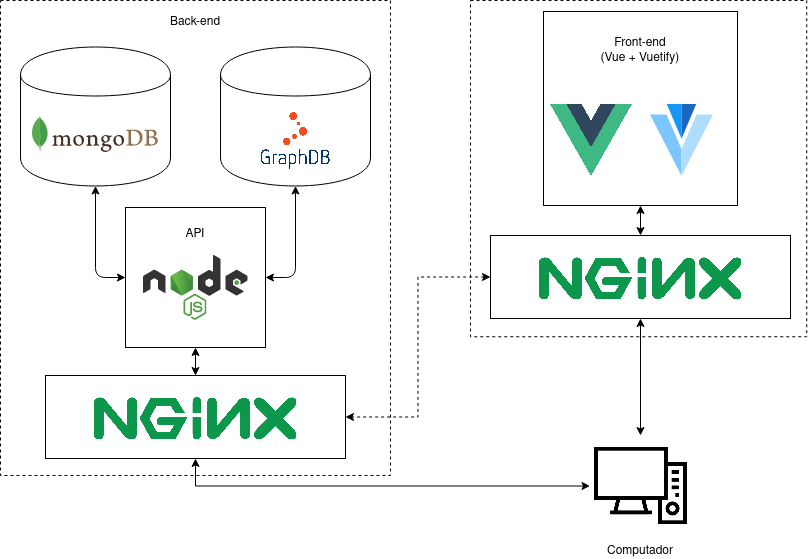
\includegraphics[width=0.9\textwidth]{img/apiHttpsArch.png}
    \caption{Arquitetura a desenvolver com \acrshort{https}}
\end{figure}

A ligação a tracejado entre os dois \textit{Nginx}'s pode ou não existir, irá depender se se pretende ou não que o servidor da interface reencaminhe pedidos para o servidor da \acrshort{api} de dados.

\section{\acrshort{api} Gateway}

Nesta secção é escolhida a tecnologia \textit{\acrshort{api} Gateway} a usar de acordo com os requisitos necessários.

Apresenta-se de seguida os requisitos que a \textit{\acrshort{api} Gateway} deve possuir:
\begin{itemize}
    \item Ser gratuita e \textit{open-source}
    \item Suportar \acrshort{https}, \acrshort{cors} e \acrshort{jwt}
    \item Suportar Autenticação e Autorização personalizada (Criação de \textit{plugin}/middleware)
    \item Possível automatização ao definir apenas ficheiros de configuração sem qualquer uso de \acrshort{cli}s, \acrshort{gui}s ou \acrshort{api}s
    \item Suportar \textit{deployment} em \textit{Docker}
    \item Suportar \textit{rate limit} e \textit{cache}
    \item Suportar versionamento da \acrshort{api}
    \item Balanceamento de carga e servir de \textit{reverse proxy}
    \item \textit{Logs} e métricas
    \item Integração da documentação desenvolvida na especificação \textit{OpenAPI}
\end{itemize}

Antes de fazer uma comparação entre as várias \textit{\acrshort{api} Gateway}s exploradas no estado de arte (~\ref{sec:api_gateway}) há uma que é imediatamente descartada, a \textit{Moleculer \acrshort{api} Gateway}. Esta \textit{\acrshort{api} Gateway} tem um melhor caso de uso quando a(s) \acrshort{api}(s) desenvolvida(s) usam a \textit{framework} \textit{Moleculer}. Como este não é o caso da \acrshort{clav} não teremos em consideração esta \textit{\acrshort{api} Gateway} na próxima tabela.

\begin{table}[H]
    \footnotesize
    \centering
    \begin{tabular}{|>{\centering\arraybackslash}p{0.3\textwidth}|>{\centering\arraybackslash}p{0.14\textwidth}|>{\centering\arraybackslash}p{0.14\textwidth}|>{\centering\arraybackslash}p{0.14\textwidth}|>{\centering\arraybackslash}p{0.14\textwidth}|}
    \hline
        Requisito & \textit{Nginx} & \textit{Kong} & \textit{Tyk} & \textit{Express Gateway} \\ \hline
        Ser gratuita e \textit{open-source} & {\color{green}\ding{52}} & {\color{green}\ding{52}} & {\color{green}\ding{52}} & {\color{green}\ding{52}} \\ \hline
        Suportar \acrshort{https}, \acrshort{cors} e \acrshort{jwt} & \acrshort{jwt} apenas na versão paga. Necessário usar \textit{plugin} & {\color{green}\ding{52}} & {\color{green}\ding{52}} & {\color{green}\ding{52}} \\ \hline
        Suportar Autenticação e Autorização personalizada (Criação de \textit{plugin}/middleware) & {\color{green}\ding{52}} (em \textit{Lua}) & {\color{green}\ding{52}} (em \textit{Lua} ou \textit{Go}) & {\color{green}\ding{52}} (em \textit{Python}, \textit{Lua} ou \textit{Javascript}) & {\color{green}\ding{52}} (em \textit{Javascript}) \\ \hline
        Possível automatização do \textit{deployment} ao definir apenas ficheiros de configuração sem qualquer uso de \acrshort{cli}s, \acrshort{gui}s ou \acrshort{api}s & {\color{green}\ding{52}} & {\color{green}\ding{52}} & {\color{red}\ding{54}} & {\color{green}\ding{52}} \\ \hline
        Suportar deployment em \textit{Docker} & {\color{green}\ding{52}} & {\color{green}\ding{52}} & {\color{green}\ding{52}} & {\color{green}\ding{52}} \\ \hline
        Suportar \textit{rate limit} e \textit{cache} & {\color{green}\ding{52}} & {\color{green}\ding{52}} & {\color{green}\ding{52}} & Não possui \textit{cache} \\ \hline
        Suportar versionamento da \acrshort{api} & {\color{red}\ding{54}} & {\color{red}\ding{54}} & {\color{green}\ding{52}} & {\color{red}\ding{54}} \\ \hline
        Balanceamento de carga e servir de \textit{reverse proxy} & {\color{green}\ding{52}} & {\color{green}\ding{52}} & {\color{green}\ding{52}} & {\color{green}\ding{52}} \\ \hline
        \textit{Logs} e métricas & {\color{green}\ding{52}} & {\color{green}\ding{52}} & {\color{green}\ding{52}} & {\color{green}\ding{52}} \\ \hline
        Integração da documentação desenvolvida na especificação \textit{OpenAPI} & {\color{red}\ding{54}} & {\color{red}\ding{54}} & {\color{green}\ding{52}} & {\color{red}\ding{54}} \\ \hline
    \end{tabular}
    \caption{Comparação entre \textit{\acrshort{api} Gateway}s~\cite{compAPIGat,kong,tyk}}
    \label{table:APIGateway}
\end{table}

Infelizmente nenhuma das tecnologias suporta todos os requisitos. Assim a partir da tabela~\ref{table:APIGateway} irá ser escolhida a tecnologia a usar tendo em conta a importância de cada requisito.

Das quatro tecnologias presentes na tabela, podemos desde já descartar o \textit{Tyk} visto não permitir automatizar o \textit{deployment}. Sobram, assim, o \textit{Nginx}, o \textit{Kong} e o \textit{Express Gateway}. Destas três, verifica-se que a última possui menos funcionalidades e portanto não será a tecnologia escolhida.

Entre o \textit{Nginx} e o \textit{Kong} a escolha irá prender-se com a facilidade e poder de configuração visto que os requisitos presentes em cada tecnologia são muito semelhantes. O \textit{Kong} é construído a partir do \textit{Nginx} (daí as suas parecenças em termos de requisitos presentes) e é possível configurar o \textit{Nginx} a partir do \textit{Kong}. Para além disso, o \textit{Kong} possui vários \textit{plugins} por forma a permitir certas funcionalidades que no \textit{Nginx} seria necessário configurar manualmente para atingir essas funcionalidades. Portanto a escolha tecnológica para a \textit{\acrshort{api} Gateway} recai sobre o \textit{Kong}.

\subsection{Arquitetura}

Após a escolha da \textit{\acrshort{api} Gateway} a usar (\textit{Kong}) é necessário proceder ao esboço de uma arquitetura base a desenvolver. Esta arquitetura apresenta-se de seguida, onde apenas se inclui a \acrshort{api} visto a interface não sofrer qualquer alteração:
\begin{figure}[H]
    \centering
    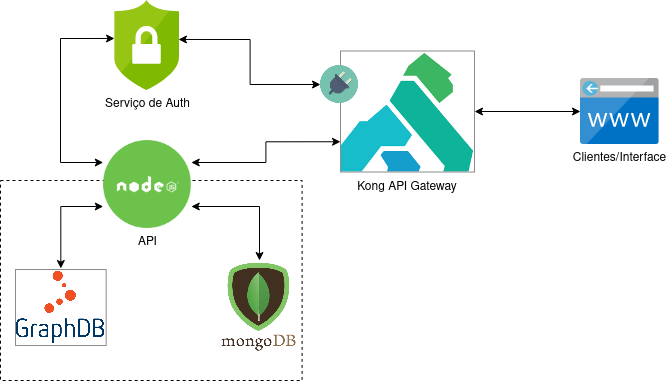
\includegraphics[width=1\textwidth]{img/apiGatewayArch.png}
    \caption{Arquitetura a desenvolver com \textit{\acrshort{api} Gateway}}\label{fig:apiGatewayArch}
\end{figure}

Apesar das várias vantagens do \textit{Kong} não é possível, através dos \textit{plugins} fornecidos por este, realizar uma proteção das rotas semelhante à presente na \acrshort{api} de dados da \acrshort{clav}. Portanto, com o intuito de simplificar a \acrshort{api} de dados, a ideia passa por retirar da \acrshort{api} de dados da \acrshort{clav} tudo que envolva proteção desta, tais como a verificação de \textit{tokens} (autenticação), a geração de \textit{tokens} bem como a verificação da autorização de um utilizador (verificar se o nível do utilizador é suficiente para aceder determinada rota), e colocar estas funcionalidades noutro servidor independente da \acrshort{api} de dados. Este servidor está representado na arquitetura como Serviço de \textit{Auth} que procederá então à autenticação e autorização dos pedidos realizados pelos clientes.

Com esta separação a \acrshort{api} de dados precisará de realizar pedidos ao Serviço de \textit{Auth} para a verificação e geração de \textit{tokens} em casos particulares como o \textit{login} de um utilizador ou a \textit{criação} de uma Chave \acrshort{api}.

Todos os pedidos realizados pelos clientes e pela interface da \acrshort{clav} tem como ponto de entrada o \textit{Kong}. Este, através de um \textit{plugin}, para cada pedido recebido irá realizar um pedido ao Serviço de \textit{Auth} onde:

\begin{enumerate}
    \item Verifica-se quem pode aceder (que tipo de clientes) à rota do pedido
    \item Procede-se à autenticação do pedido (se necessário)
    \item Procede-se à autorização do pedido (se necessário)
\end{enumerate}

Caso a resposta do Serviço de \textit{Auth} seja positiva então o \textit{Kong} procederá à realização do pedido à \acrshort{api} de dados. Caso contrário, o pedido à \acrshort{api} de dados não é efetuado e é devolvido ao utilizador a resposta de erro correspondente (erro de autenticação ou de autorização).

\section{Resumo}

Este capítulo tem como principal objetivo tornar mais fácil a compreensão das várias decisões tomadas descrevendo os vários requisitos a cumprir. Além disso, apresenta-se também com base nessas decisões uma arquitetura/modelo inicial da solução a desenvolver. Foram assim abordados a proteção da \acrshort{api} de dados, a autenticação através de \acrfull{cmd}, a documentação da \acrshort{api} de dados, a migração de \acrshort{http} para \acrshort{https} e por fim, a \acrshort{api} Gateway.
